% \section{\appendixname~\theappendixframenumber~: Non-linear problems}\labelappendixframe{frame:nonlinear}

% \begin{frame}{Non-linear problems}
% 	TODO
% \end{frame}
% \addtocounter{appendixframenumber}{1}

\section{\appendixname~\theappendixframenumber~: Data-driven vs Physics-Informed training}\labelappendixframe{frame:datavspinns}

\begin{frame}{Problem considered}
	\textbf{Problem statement:} Consider the Poisson problem in 1D with Dirichlet BC:
	\vspace{-5pt}
	\begin{equation*}
		\left\{
		\begin{aligned}
			-\partial_{xx} u & = f, \; &  & \text{in } \; \Omega \times \mathcal{M}, \\
			u         & = 0, \;  &  & \text{on } \; \partial\Omega \times \mathcal{M},
		\end{aligned}
		\right.
		% \label{eq:Lap2D}\tag{$\mathcal{P}$}
	\end{equation*}

	\vspace{-5pt}
	with $\Omega=[0,1]^2$ and $\mathcal{M}=[0,1]^3$ ($p=3$ parameters).
		
	\vspace{4pt}
	\textbf{Analytical solution :} $\quad u(x;\bm{\mu})=\mu_1\sin(2\pi x)+\mu_2\sin(4\pi x)+\mu_3\sin(6\pi x) \,.$

	\vspace{4pt}
	\textbf{Construction of two priors:} MLP of 6 layers; Adam optimizer (10000 epochs). \\
	Imposing the Dirichlet BC exactly in the PINN with $\varphi(x)=x(x-1)$.

	\begin{itemize}
		\item \textbf{Physics-informed training:} $N_\text{col}=5000$ collocation points.
		$$J_r(\theta) \simeq
			\frac{1}{N_\text{col}} \sum_{i=1}^{N_\text{col}} \big| \partial_{xx}u_\theta(\bm{x}_\text{col}^{(i)};\bm{\mu}_\text{col}^{(i)}\big) + f\big(\bm{x}_\text{col}^{(i)};\bm{\mu}_\text{col}^{(i)}\big) \big|^2.$$
	
		\item \textbf{Data-driven training:}  $N_\text{data}=5000$ data.
		$$J_\text{data}(\theta) =
		\frac{1}{N_\text{data}}
		\sum_{i=1}^{N_\text{data}} \big| u_\theta^\text{data}(\bm{x}_\text{data}^{(i)};\bm{\mu}_\text{data}^{(i)}) - u(\bm{x}_\text{data}^{(i)};\bm{\mu}_\text{data}^{(i)}) \big|^2.$$
	\end{itemize}
\end{frame}

\begin{frame}{Priors derivatives}
	\vspace{-10pt}
	$$\bm{\mu}^{(1)}=(0.3,0.2,0.1)$$
	\begin{figure}[ht!]
		\centering
		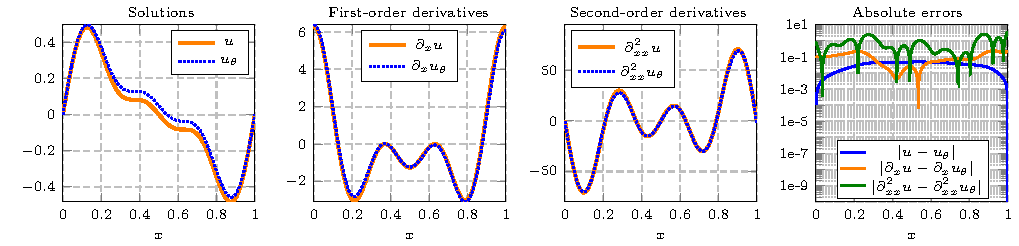
\includegraphics[width=\linewidth]{images/appendix/datavspinns/standalone_solutions_and_errors_PINN.pdf}
	\end{figure}
	
	\begin{figure}[ht!]
		\centering
		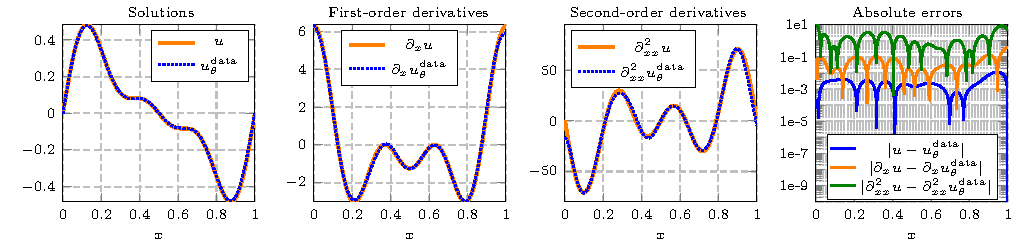
\includegraphics[width=\linewidth]{images/appendix/datavspinns/standalone_solutions_and_errors_NN.pdf}
	\end{figure}
\end{frame}

\begin{frame}{Additive approach in $\mathbb{P}_1$}
	\vspace{-2pt}
	\textbf{1 set of parameters:} $\quad \bm{\mu}^{(1)}=(0.3,0.2,0.1)$
	
	\begin{table}[H]
		\centering
		\gainsbothNN{images/appendix/datavspinns/FEM_param1.csv}{images/appendix/datavspinns/compare_gains_param1.csv}
	\end{table}

	\vspace{6pt}
	\textbf{50 set of parameters:}

	\begin{table}[H]
		\centering
		\gainstableMult{images/appendix/datavspinns/Tab_stats_case1_degree1.csv}
	\end{table}

	\footnotesize
	$N$ : Nodes.
\end{frame}

\addtocounter{appendixframenumber}{1}

\section{\appendixname~\theappendixframenumber~: Multiplicative approach}\labelappendixframe{frame:mult}

\begin{frame}{Multiplicative approach}
	\textbf{Liffted problem :} Considering $M$ such that $u_M=u+M>0$ on $\Omega$,
	\begin{equation*}
		% \label{eq:ob_pde_M}
		\begin{dcases}
			\mathcal{L}(u_M)=f, &
			\text{\quad in } \Omega,          \\
			u_M = M,                  &
			\text{\quad on } \partial \Omega. \\
		\end{dcases}
	\end{equation*}

	\textbf{Variational Problem :} Let $u_{\theta,M}=u_\theta+M \in M + H^{k+1}(\Omega)\cap H^1_0(\Omega)$.
	
	\vspace{-5pt}
	\begin{equation}
		\label{eq:weaktimes}
		\text{Find } p_h^\times \in 1 + V_h^0 \text{ such that}, \forall v_h \in V_h^0, a \big(u_{\theta,M} \; p_h^\times,u_{\theta,M}  v_h \big) = l(u_{\theta,M} v_h),\tag{$\mathcal{P}_h^\times$}
	\end{equation}

	\vspace{5pt}
	\begin{minipage}[t]{0.6\linewidth}
		with the \textcolor{red}{enriched trial space $V_h^\times$} defined by
		\begin{equation*}
			\left\{
			u_{h,M}^\times = u_{\theta,M} \; p_h^\times,
			\quad p_h^\times \in 1+V_h^0
			\right\}.
		\end{equation*}
	
		\vspace{2pt}
		\textbf{General Dirichlet BC :} If $u=g$ on $\partial \Omega$, then
		\[
			p_h^\times = \frac{g+M}{u_{\theta,M}} \text{\quad on } \partial \Omega,
		\]
		with $u_{\theta,M}$ the PINN prior. 
	\end{minipage} 
	% \qquad \begin{minipage}[t][][b]{0.28\linewidth}
	% 	\vspace{-8pt}
	% 	\centering
	% 	\pgfimage[width=\linewidth]{images/correction/correction.pdf}
	% \end{minipage}
\end{frame}

\begin{frame}{Convergence analysis}
	\hypersetup{
		citecolor=white,
	}

	\begin{mytheo}{Convergence analysis of the enriched FEM \footnotesize\citep{ours_2025}\normalsize}{mult}
		We denote $u_{h,M}^\times \in V_h^\times$ the solution of \eqref{eq:weaktimes} with $V_h^\times$ the enriched trial space. Then, denoting $u_h^\times=u_{h,M}^\times-M$,
		\vspace{-5pt}
		\begin{equation*}
			| u-u_h^\times|_{H^1} \leqslant \fcolorbox{red}{other!10!white}{$\left| \frac{u_M}{u_{\theta,M}} \right|_{H^{q+1}} \frac{\| u_{\theta,M}\|_{W^{1,\infty}}}{| u |_{H^{q+1}}}$} \left(C_{H^1} \, h^{k} |u|_{H^{k+1}}\right),
		\end{equation*}
		\begin{equation*}
			\| u-u_h^\times\|_{L^2} \leqslant \fcolorbox{red}{other!10!white}{$C_{\theta,M}\left| \frac{u_M}{u_{\theta,M}} \right|_{H^{q+1}} \frac{\| u_{\theta,M}\|_{W^{1,\infty}}^2}{| u |_{H^{q+1}}}$} \left(C_{L^2} \, h^{k+1} |u|_{H^{k+1}}\right).
		\end{equation*}
		with
		\begin{equation*}
			C_{\theta,M}=\|u_{\theta,M}^{-1}\|_{L^{\infty}}
			+2|u_{\theta,M}^{-1}|_{W^{1,\infty}}
			+|u_{\theta,M}^{-1}|_{W^{2,\infty}}.
		\end{equation*}
	\end{mytheo}

	\hypersetup{
		citecolor=other,
	}
\end{frame}

\begin{frame}{Comparison of the two enriched methods}
	\hypersetup{
		citecolor=white,
	}

	\begin{mytheo}{\footnotesize\citep{ours_2025}\normalsize}{addvsmult}
		We have
		\begin{equation*}
			\fcolorbox{red}{other!10!white}{$\left| \frac{u_M}{u_{\theta,M}} \right|_{H^{q+1}} \frac{\| u_{\theta,M}\|_{W^{1,\infty}}}{| u |_{H^{q+1}}}$}
			\underset{M\rightarrow\infty}{\longrightarrow}
			\fcolorbox{orange}{other!10!white}{$\frac{| u-u_{\theta} |_{H^{k+1}}}{| u |_{H^{k+1}}}$},
		\end{equation*}
		in $H^1$ semi-norm and
		\begin{equation*}
			\fcolorbox{red}{other!10!white}{$C_{\theta,M}\left| \frac{u_M}{u_{\theta,M}} \right|_{H^{q+1}} \frac{\| u_{\theta,M}\|_{W^{1,\infty}}^2}{| u |_{H^{q+1}}}$}
			\underset{M\rightarrow\infty}{\longrightarrow}
			\fcolorbox{orange}{other!10!white}{$\frac{| u-u_{\theta} |_{H^{k+1}}}{| u |_{H^{k+1}}}$},
		\end{equation*}
		in $L^2$ norm.
	\end{mytheo}

	\textcolor{red}{Multiplicative} and \textcolor{orange}{Additive} approaches.
	\hypersetup{
		citecolor=other,
	}
\end{frame}

\begin{frame}{Numerical results}
	Considering the 1D Poisson problem of \refappendix{frame:datavspinns}.

	\textbf{Error estimates :} 1 set of parameters.
		$$\bm{\mu}^{(1)}=(0.3,0.2,0.1) $$
		
		\vspace{-15pt}
		\begin{figure}[H]
		\cvgFEMCorrMultOnedeg{images/appendix/mult/FEM_case1_v1_param1_degree1.csv}{images/appendix/mult/FEM_case1_v1_param1_degree2.csv}{images/appendix/mult/Corr_case1_v1_param1_degree1.csv}{images/appendix/mult/Mult_case1_v1_param1_degree1_M3.0.csv}{images/appendix/mult/Mult_case1_v1_param1_degree1_M100.0.csv}{1e-5}
	\end{figure}
\end{frame}

\addtocounter{appendixframenumber}{1}